\begin{figure}

		\centering
		
		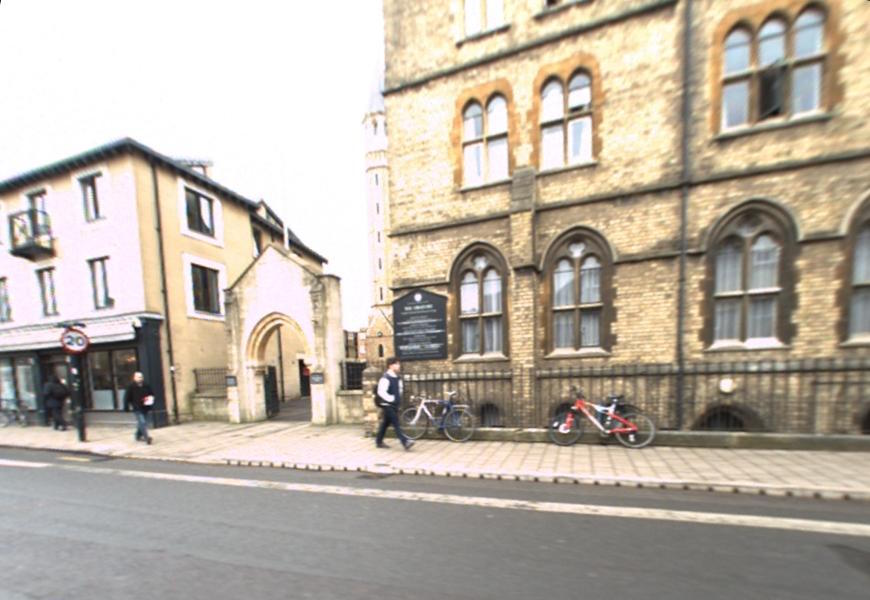
\includegraphics[width=0.33\linewidth]{details/image0.jpg}\hfill
		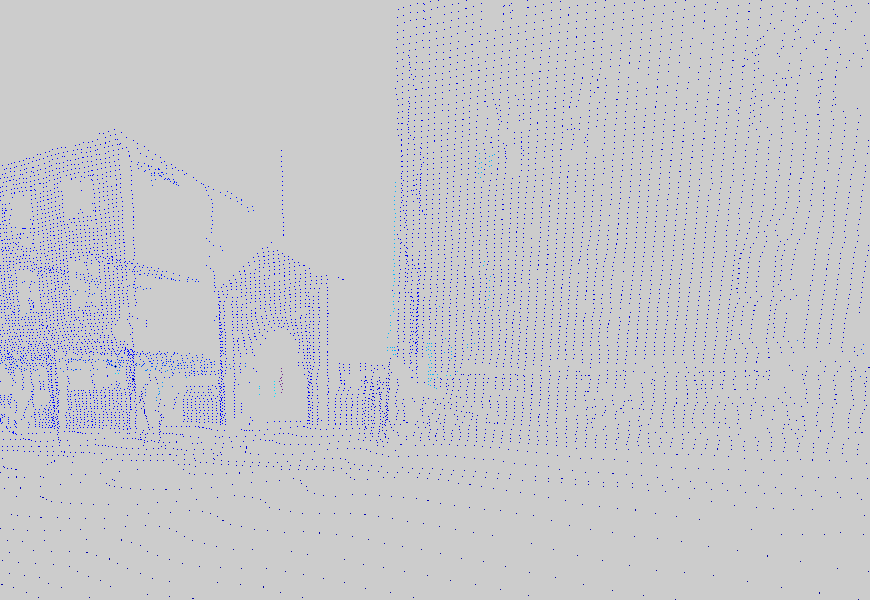
\includegraphics[width=0.33\linewidth]{details/sparsedepth0.png}\hfill
		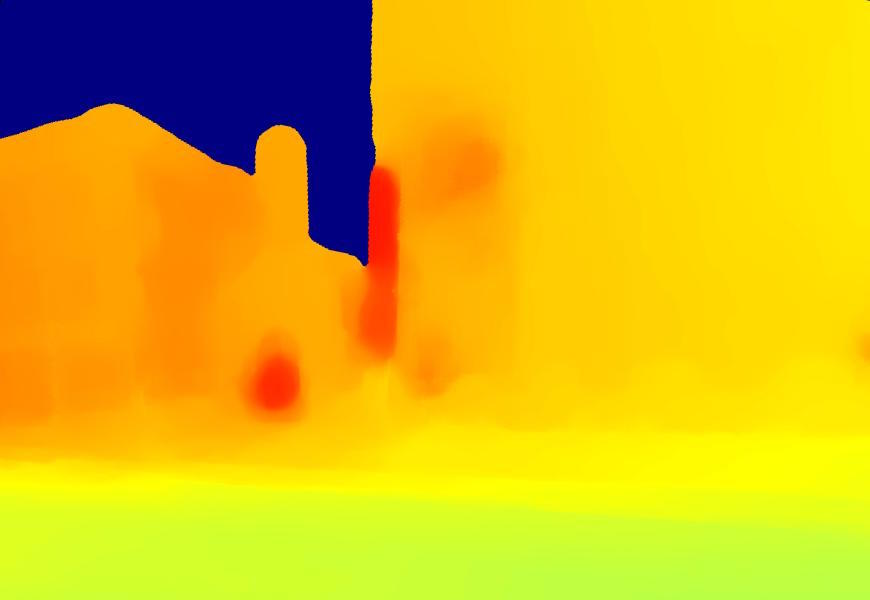
\includegraphics[width=0.33\linewidth]{details/densedepth0.jpg}\hfill
		
		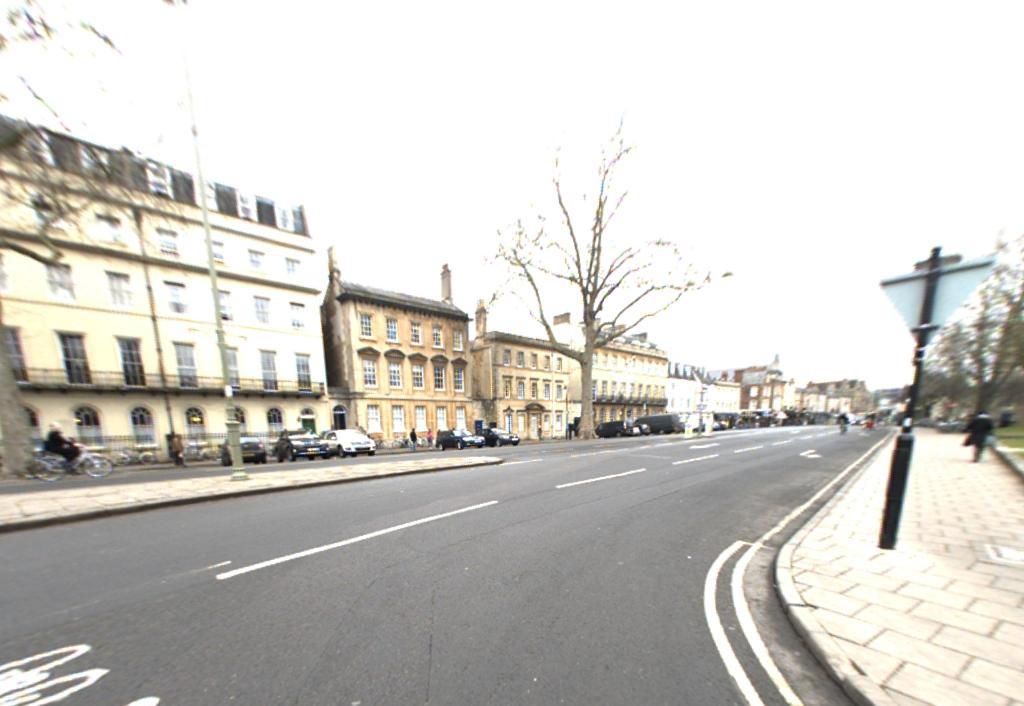
\includegraphics[width=0.33\linewidth]{details/image1.jpg}\hfill
		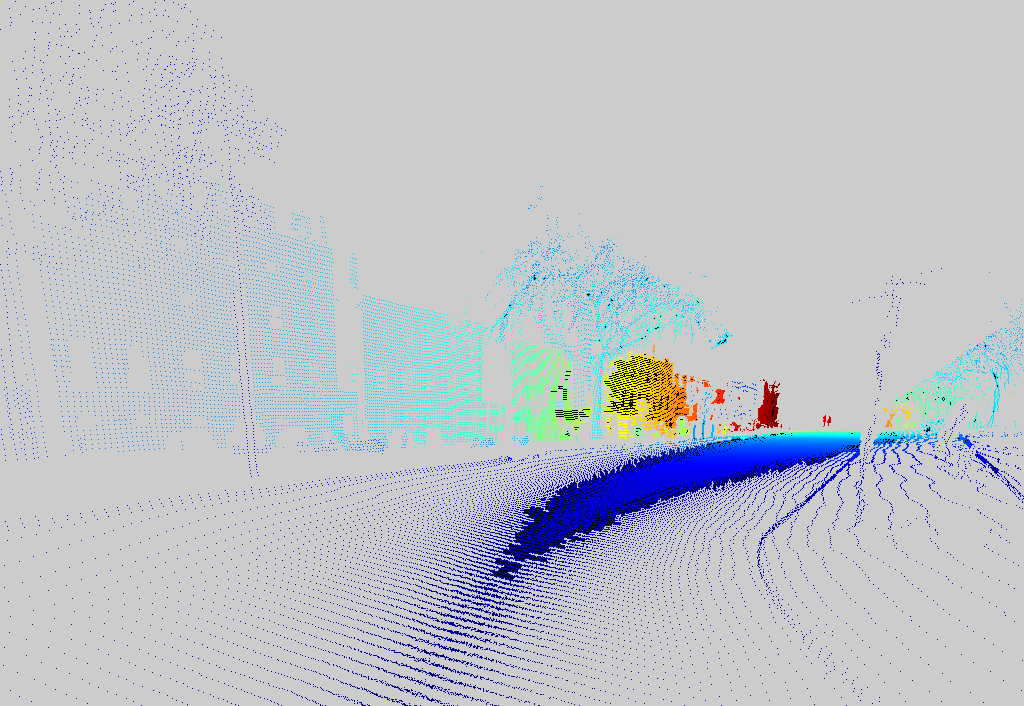
\includegraphics[width=0.33\linewidth]{details/sparsedepth1.png}\hfill
		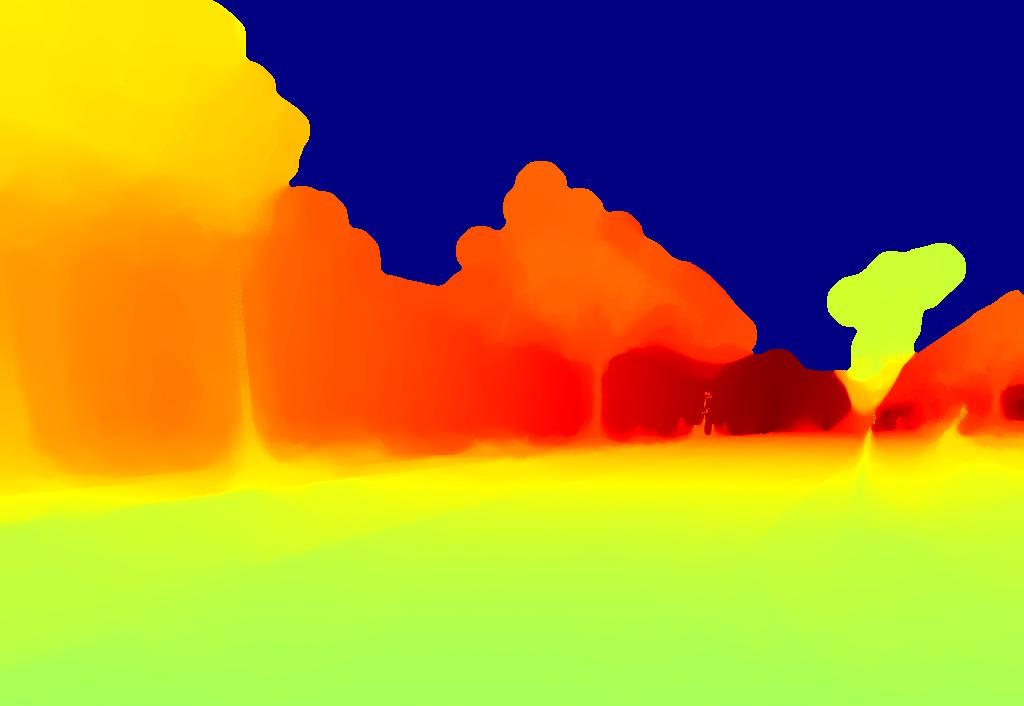
\includegraphics[width=0.33\linewidth]{details/densedepth1.jpg}\hfill
		\caption[Point cloud to depth map]{\label{fig:depth_map} \textbf{From point cloud to dense depth map:} from left to right: raw image, point cloud viewed from the camera frame, inpainted depth map by~\citep{Bevilacqua2017} (\textcolor{green}{green} is near, \textcolor{red}{red} is far).}

\end{figure}
	